% Created 2020-02-18 Tue 22:10
% Intended LaTeX compiler: pdflatex
\documentclass[11pt]{article}
\usepackage[utf8]{inputenc}
\usepackage[T1]{fontenc}
\usepackage{graphicx}
\usepackage{grffile}
\usepackage{longtable}
\usepackage{wrapfig}
\usepackage{rotating}
\usepackage[normalem]{ulem}
\usepackage{amsmath}
\usepackage{textcomp}
\usepackage{amssymb}
\usepackage{capt-of}
\usepackage{hyperref}
\usepackage{minted}
\usepackage{amsmath}
\usepackage{esint}
\usepackage[english, russian]{babel}
\usepackage{mathtools}
\usepackage{amsthm}
\usepackage[top=0.8in, bottom=0.75in, left=0.625in, right=0.625in]{geometry}
\def\zall{\setcounter{lem}{0}\setcounter{cnsqnc}{0}\setcounter{th}{0}\setcounter{Cmt}{0}\setcounter{equation}{0}}
\newcounter{lem}\setcounter{lem}{0}
\def\lm{\par\smallskip\refstepcounter{lem}\textbf{\arabic{lem}}}
\newtheorem*{Lemma}{Лемма \lm}
\newcounter{th}\setcounter{th}{0}
\def\th{\par\smallskip\refstepcounter{th}\textbf{\arabic{th}}}
\newtheorem*{Theorem}{Теорема \th}
\newcounter{cnsqnc}\setcounter{cnsqnc}{0}
\def\cnsqnc{\par\smallskip\refstepcounter{cnsqnc}\textbf{\arabic{cnsqnc}}}
\newtheorem*{Consequence}{Следствие \cnsqnc}
\newcounter{Cmt}\setcounter{Cmt}{0}
\def\cmt{\par\smallskip\refstepcounter{Cmt}\textbf{\arabic{Cmt}}}
\newtheorem*{Note}{Замечание \cmt}
\renewcommand{\div}{\operatorname{div}}
\newcommand{\rot}{\operatorname{rot}}
\newcommand{\grad}{\operatorname{grad}}
\author{Sergey Makarov}
\date{\today}
\title{}
\hypersetup{
 pdfauthor={Sergey Makarov},
 pdftitle={},
 pdfkeywords={},
 pdfsubject={},
 pdfcreator={Emacs 26.3 (Org mode 9.3)}, 
 pdflang={English}}
\begin{document}

\zall

ДЗ: 12.5, 12.7
\begin{equation}
\begin{cases}
u_{tt} = 4u_{xx} + xt, \\
u(x, 0) = x^2, \\
u_t(x, 0) = x.
\end{cases}
\end{equation}
\begin{equation}
\begin{cases}
u_{tt} = u_{xx} + \sin t, \\
u(x, 0) = \sin x, \\
u_t(x, 0) = \cos x.
\end{cases}
\end{equation}
\begin{equation}
\begin{cases}
u_{tt} = u_{xx}, \\
u(x, 0) = \begin{cases}
\cos x, |x| < \frac{\pi}2, \\
0, |x| > \frac{\pi}2.
\end{cases}
u_t(x, 0) = 0
\end{cases}
\end{equation}
В последнем случае найти $u\left(x, \frac{\pi}4\right)$
\begin{equation}
\begin{cases}
u_{tt} = u_{xx}, \\
u(x, 0) = 0, \\
u_t(x, 0) = \begin{cases}
\cos x, |x| < \frac{\pi}2, \\
0, |x| > \frac{\pi}2.
\end{cases}
\end{cases}
\end{equation}
\textbf{Формула д'Аламбера}:
\begin{equation}
u(x, t) = \frac12(\varphi(x + at) + \varphi(x - at)) +
\frac1{2a}\int_{x - at}^{x + at}\varphi(\xi)d\xi +
\frac1{2a}\int_0^l\int_{x - a(t - \tau)}^{x + a(t - \tau)}f(\xi, \tau)d\xi d\tau
\end{equation}
\section{Задача 12.5}
\label{sec:org2e65491}
\begin{equation}
\begin{cases}
u_{tt} = a^2u_{xx}, -\infty < x < +\infty, t > 0, a > 0, \\
u(x, 0) = \begin{cases}
1 - \frac{|x|}c, |x| \leq c, \\
0, |x| > c, \\
\end{cases}
u_t(x, 0) = 0.
\end{cases}
\end{equation}
$u(x)$ при фиксированном $t > 0$ - ?
\subsection{Решение}
\label{sec:orgeab4a70}
\begin{center}
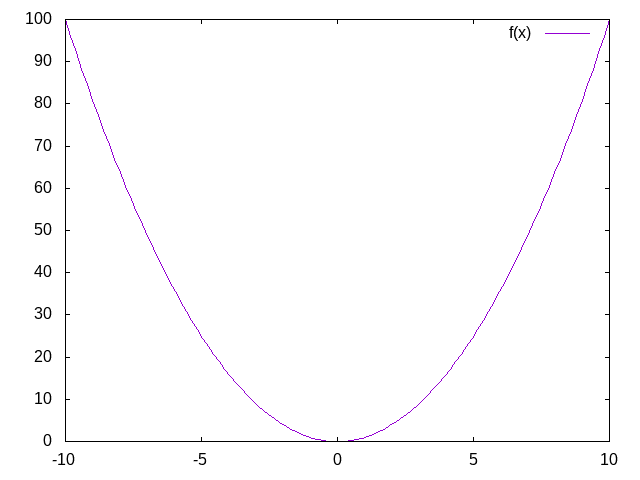
\includegraphics[width=.9\linewidth]{img/res.png}
\end{center}
\end{document}
